\documentclass[UTF8,a4paper,12pt]{ctexart}

\usepackage{geometry}
\geometry{left=2.5cm,right=2.5cm,top=2.6cm,bottom=2.6cm}

\usepackage{graphicx}
\usepackage{float}
\usepackage{booktabs}
\usepackage{longtable}
\usepackage{array}
\usepackage{multirow}
\usepackage{caption}
\usepackage{subcaption}
\usepackage{amsmath}
\usepackage{amssymb}
\usepackage{listings}
\usepackage{xcolor}
\usepackage{hyperref}
\usepackage{url}
\usepackage{setspace}

\hypersetup{
    colorlinks=true,
    linkcolor=black,
    urlcolor=blue,
    citecolor=black
}

\setstretch{1.25}

\lstset{
    language=Python,
    basicstyle=\ttfamily\small,
    keywordstyle=\color{blue},
    commentstyle=\color{gray},
    stringstyle=\color{teal},
    numbers=left,
    numberstyle=\tiny,
    stepnumber=1,
    numbersep=8pt,
    frame=single,
    breaklines=true,
    tabsize=4,
    showstringspaces=false
}

\title{\textbf{Group Discovery：基于 students003 行人轨迹数据的逐帧聚类与可视化实验报告}}
\author{姓名： \quad 学号：}
\date{\today}

\begin{document}

\maketitle

\begin{abstract}
本文围绕 students003 行人轨迹数据完成 Group Discovery 实验。实验目标是在每一帧中对行人轨迹坐标点进行聚类，自动发现行人组，并使用不同颜色可视化不同组，最终生成完整视频。本文首先对数据格式、时间步、行人数量和坐标范围进行检查；随后按照由浅入深的实验主线，依次设计并实现了 A 类基础单帧空间聚类、B 类运动特征增强、C 类时序关系建模以及 D 类参数分析与稳定性评价。A 类方法仅使用二维位置坐标作为 baseline；B 类方法进一步引入瞬时速度、滑动窗口速度、指数动量和运动方向；C 类方法从行人两两关系角度构造持续邻近关系、关系图和 pairwise affinity。由于数据集未提供真实行人组标签，本文不采用准确率、召回率和 F1 等监督指标，而使用平均簇数量、噪声点比例、运行时间、连续帧稳定性以及可视化结果进行综合评价。最终，本文选择基于滑动窗口速度特征的 DBSCAN + KMeans 兜底策略作为 Final 方法。实验结果表明，最终方法覆盖全部 541 帧，平均每帧得到约 3.95 个行人组，所有帧均满足至少 2 个行人组的要求，并成功生成最终 MP4 视频。
\end{abstract}

\noindent\textbf{关键词：} Group Discovery；行人轨迹聚类；DBSCAN；KMeans 兜底；运动特征；时序关系建模；可视化

\newpage
\tableofcontents
\newpage

\section{引言}

Group Discovery 任务的目标是从行人轨迹数据中自动发现具有相似空间位置或运动关系的行人组。与普通监督分类任务不同，本实验数据未提供真实行人组标签，因此需要在无监督条件下进行聚类分析、可视化展示和结果评价。

本实验使用 students003 数据，对视频中每一帧的行人轨迹坐标点进行聚类，并用不同颜色标记不同的行人组，最终生成 MP4 视频。根据作业要求，实验需要满足以下条件：使用 students003 数据；对每一帧行人坐标点进行聚类；自动发现行人组；不同颜色表示不同组；形成视频；每帧至少显示 2 组行人；报告按照正式实验报告或学术论文规范撰写，并包含关键代码。

为避免只进行简单的 KMeans 或 DBSCAN 对比，本文按照 A/B/C/D/Final 的实验主线逐步推进：A 类方法建立单帧空间聚类 baseline；B 类方法引入运动特征；C 类方法引入时序关系建模；D 类方法进行参数分析和稳定性评价；Final 方法在综合比较后生成最终视频。

\section{数据集与任务要求}

\subsection{数据格式}

students003 数据集中每条记录包含四个字段：
\begin{equation}
    (time\_step, ID, X, Y)
\end{equation}
其中，\texttt{time\_step} 表示时间步或帧编号，\texttt{ID} 表示行人编号，\texttt{X} 和 \texttt{Y} 表示该行人在二维平面中的位置坐标。

数据检查结果如表 \ref{tab:dataset-summary} 所示。

\begin{table}[H]
\centering
\caption{students003 数据集统计结果}
\label{tab:dataset-summary}
\begin{tabular}{ll}
\toprule
统计项 & 数值 \\
\midrule
轨迹记录数 & 17953 \\
时间步数量 & 541 \\
行人 ID 数量 & 434 \\
时间步范围 & 0 到 5400 \\
时间步间隔 & 10 \\
每帧最少行人数 & 13 \\
每帧最多行人数 & 52 \\
每帧平均行人数 & 约 33.18 \\
缺失值数量 & 0 \\
重复 \texttt{time\_step, ID} 记录 & 0 \\
\bottomrule
\end{tabular}
\end{table}

数据检查表明，students003 数据时间步连续，且每一帧均包含多个行人点，能够满足逐帧聚类和视频可视化实验要求。

\subsection{任务要求理解}

对于每一帧 $t$，本文取出该帧中所有行人的坐标点：
\begin{equation}
P_t = \{(x_i, y_i)\}_{i=1}^{n_t}
\end{equation}
并对 $P_t$ 进行聚类，得到每个行人的组标签。最终可视化时，不同组使用不同颜色表示，点旁标注行人 ID，并将所有帧合成为视频。

需要注意的是，数据中没有真实的行人组标签，因此本文不使用监督评价指标，而采用无监督统计指标和可视化分析进行评价。

\section{方法设计}

\subsection{A 类：基础单帧空间聚类}

A 类方法只使用每一帧的二维坐标：
\begin{equation}
[X, Y]
\end{equation}
作为聚类输入。本文实现了 KMeans、DBSCAN、Agglomerative Clustering 和 GMM 四种基础方法。其中，KMeans、Agglomerative Clustering 和 GMM 需要预先指定簇数量；DBSCAN 不需要指定簇数量，能够根据局部密度自动发现行人组，并可将孤立点标记为噪声点。

A 类方法的作用是建立 baseline，用于回答仅依赖当前帧空间位置是否能够初步发现行人组。

\subsection{B 类：运动特征增强}

A 类方法只考虑当前位置，无法表达行人是否具有相似运动趋势。因此，B 类方法在 $X,Y$ 坐标基础上加入运动特征。

瞬时速度定义为：
\begin{equation}
v_x(t)=\frac{x(t)-x(t-\Delta t)}{\Delta t},\quad
v_y(t)=\frac{y(t)-y(t-\Delta t)}{\Delta t}
\end{equation}

滑动窗口速度定义为：
\begin{equation}
v_x^{win}(t)=\frac{x(t)-x(t-w)}{t-(t-w)},\quad
v_y^{win}(t)=\frac{y(t)-y(t-w)}{t-(t-w)}
\end{equation}

指数动量特征定义为：
\begin{equation}
m_t=\alpha m_{t-1}+(1-\alpha)v_t
\end{equation}

运动方向用 $\cos\theta,\sin\theta$ 表示，以避免角度周期问题：
\begin{equation}
\theta=\arctan2(v_y,v_x)
\end{equation}

本文分别实验以下 B 类特征：

\begin{itemize}
    \item 位置 + 瞬时速度：$[X,Y,v_x,v_y]$
    \item 位置 + 滑动窗口速度：$[X,Y,window\_v_x,window\_v_y]$
    \item 位置 + 指数动量：$[X,Y,momentum\_v_x,momentum\_v_y]$
    \item 位置 + 运动方向：$[X,Y,\cos\theta,\sin\theta]$
\end{itemize}

\subsection{C 类：时序关系建模}

A 类和 B 类方法的基本思想都是为当前帧中的每一个行人构造特征向量，然后在单帧内部进行聚类。A 类方法使用位置特征 $[X,Y]$，B 类方法进一步加入速度、滑动窗口速度或动量等运动特征。虽然这些方法能够反映当前帧中的空间邻近关系和局部运动趋势，但它们仍然主要从“单个行人特征”的角度进行建模，对“两个行人是否在一段时间内持续同行”这一关系表达不够直接。

在 Group Discovery 任务中，一组同行行人通常不仅在某一帧中距离较近，而且会在连续多个时间步中保持相对接近，并具有相似的运动方向或速度变化。因此，本文进一步设计 C 类时序关系建模方法，将研究重点从单个行人的特征表示转向行人与行人之间的 pairwise relation，即直接刻画任意两名行人在最近时间窗口内的持续邻近程度和运动相似性。

设当前帧为 $t$，行人 $i$ 和行人 $j$ 在时间窗口 $\mathcal{T}_t$ 内共同出现，则两人之间的平均空间距离定义为：
\[
D_{ij}^{pos}(t)=\frac{1}{|\mathcal{T}_{ij}|}
\sum_{\tau\in\mathcal{T}_{ij}}
\sqrt{(x_i(\tau)-x_j(\tau))^2+(y_i(\tau)-y_j(\tau))^2},
\]
其中，$\mathcal{T}_{ij}$ 表示在最近窗口内二者同时出现的时间步集合。类似地，可以计算两人之间的平均速度差：
\[
D_{ij}^{vel}(t)=\frac{1}{|\mathcal{T}_{ij}|}
\sum_{\tau\in\mathcal{T}_{ij}}
\sqrt{(v_{x,i}(\tau)-v_{x,j}(\tau))^2+(v_{y,i}(\tau)-v_{y,j}(\tau))^2}.
\]

基于上述 pairwise relation，本文实现了三类 C 类方法。

\begin{enumerate}
    \item \textbf{持续邻近关系 + 层次聚类。}
    该方法首先根据最近时间窗口内的平均空间距离和平均速度差，构造当前帧行人之间的 pairwise distance matrix。随后使用层次聚类方法对该距离矩阵进行聚类。与 A 类单帧空间聚类相比，该方法不仅考虑当前帧距离，还引入了最近多帧中的持续邻近关系，因此能够在一定程度上减少由单帧偶然靠近造成的误分组。

    \item \textbf{基于关系图的图聚类。}
    该方法将当前帧中的每个行人视为图中的一个节点。当两名行人在最近窗口内的平均空间距离小于阈值，且平均速度差小于阈值时，在二者之间建立一条边。图中每个连通分量被视为一个行人组。该方法的优点是不需要预先指定聚类簇数，能够根据行人之间的持续邻近和运动相似关系自动形成不同数量的组；但它也对距离阈值和速度阈值较敏感，阈值过严时容易产生过度切分，阈值过松时又可能由于连通分量的传递性导致过度合并。

    \item \textbf{基于 Pairwise Affinity 的谱聚类。}
    该方法根据两名行人的平均空间距离和平均速度差构造 affinity 矩阵。两人越持续接近、运动越相似，其 affinity 值越大。本文采用如下形式构造亲和度：
    \[
    A_{ij}=
    \exp\left(-\frac{(D_{ij}^{pos})^2}{2\sigma_d^2}\right)
    \cdot
    \exp\left(-\frac{(D_{ij}^{vel})^2}{2\sigma_v^2}\right).
    \]
    随后使用谱聚类对 affinity 矩阵进行分组。该方法能够综合空间邻近和运动相似关系，但实验中仍需要指定聚类簇数，因此它更适合作为时序关系建模下的固定簇数对照方法。
\end{enumerate}

总体而言，C 类方法的主要意义在于将 Group Discovery 从“对单帧行人点进行聚类”扩展为“对行人之间的持续关系进行建模”。这使得方法能够更直接地表达同行关系。不过，C 类方法也引入了更多参数，例如时间窗口长度、距离阈值、速度阈值以及 affinity 的尺度参数等，因此后续实验需要结合统计指标和可视化结果分析其参数敏感性。

\subsection{Final 方法}

在前述 A、B、C 类方法的基础上，本文最终采用基于滑动窗口速度特征的 DBSCAN + KMeans 兜底策略作为 Final 方法。该方法的输入特征为：
\begin{equation}
[X,Y,window\_v_x,window\_v_y]
\end{equation}

其中，$X,Y$ 表示当前帧的空间位置，$window\_v_x,window\_v_y$ 表示最近时间窗口内估计得到的平均速度。本文在特征标准化后设置位置权重和运动权重，使运动特征作为空间位置的辅助信息参与聚类。

每一帧首先使用 DBSCAN 自动发现行人组；若某一帧 DBSCAN 得到的有效组数少于 2，则使用 KMeans 将该帧划分为 2 组，从而满足“每帧至少 2 组行人”的作业要求。Final 方法参数设置如表 \ref{tab:final-params} 所示。

\begin{table}[H]
\centering
\caption{Final 方法参数设置}
\label{tab:final-params}
\begin{tabular}{lc}
\toprule
参数 & 取值 \\
\midrule
\texttt{eps} & 1.0 \\
\texttt{min\_samples} & 2 \\
\texttt{window\_size} & 5 \\
\texttt{position\_weight} & 1.0 \\
\texttt{motion\_weight} & 0.5 \\
\bottomrule
\end{tabular}
\end{table}

\section{实验设置}

\subsection{实验环境}

实验在 Linux / AutoDL / Conda / Python 环境下完成。主要使用 Python 数据处理与机器学习工具库，包括 \texttt{pandas}、\texttt{numpy}、\texttt{scikit-learn}、\texttt{matplotlib} 和 \texttt{ffmpeg}。

\subsection{评价指标}

由于数据集中没有真实行人组标签，本文不使用准确率、召回率和 F1 值。采用以下指标评价聚类结果：

\begin{itemize}
    \item 平均簇数：\texttt{avg\_num\_clusters}
    \item 最小簇数和最大簇数：\texttt{min\_num\_clusters}, \texttt{max\_num\_clusters}
    \item 簇数量标准差：\texttt{std\_num\_clusters}
    \item 平均噪声比例：\texttt{avg\_noise\_ratio}
    \item 平均每帧运行时间：\texttt{avg\_runtime\_sec}
    \item 每帧至少 2 组比例：\texttt{ratio\_frames\_at\_least\_2\_clusters}
    \item 连续帧簇数量变化：\texttt{mean\_cluster\_count\_change}
\end{itemize}

其中，连续帧稳定性指标定义为：
\begin{equation}
\Delta C_t = |C_t - C_{t-1}|
\end{equation}
并统计其平均值。该值越小，说明相邻帧之间聚类组数量变化越平滑。

\section{实验结果与分析}

\subsection{A 类基础空间聚类结果}

A 类方法结果如表 \ref{tab:a-baseline} 所示。

\begin{table}[H]
\centering
\caption{A 类基础空间聚类结果}
\label{tab:a-baseline}
\begin{tabular}{lccccc}
\toprule
方法 & 平均簇数 & 最少簇数 & 最多簇数 & 噪声比例 & 至少 2 组比例 \\
\midrule
KMeans & 3.000 & 3 & 3 & 0.000 & 1.000 \\
DBSCAN & 4.652 & 2 & 8 & 0.077 & 1.000 \\
Agglomerative & 3.000 & 3 & 3 & 0.000 & 1.000 \\
GMM & 3.000 & 3 & 3 & 0.000 & 1.000 \\
\bottomrule
\end{tabular}
\end{table}

KMeans、Agglomerative Clustering 和 GMM 均固定输出 3 个簇，因此结果稳定，但不能根据每帧真实空间结构自动调整组数。DBSCAN 平均每帧得到约 4.65 个有效簇，平均噪声比例约为 7.7\%，更符合自动发现组数的任务目标。

图 \ref{fig:a-dbscan} 展示了 A 类 DBSCAN 在关键帧上的结果。

\begin{figure}[H]
\centering
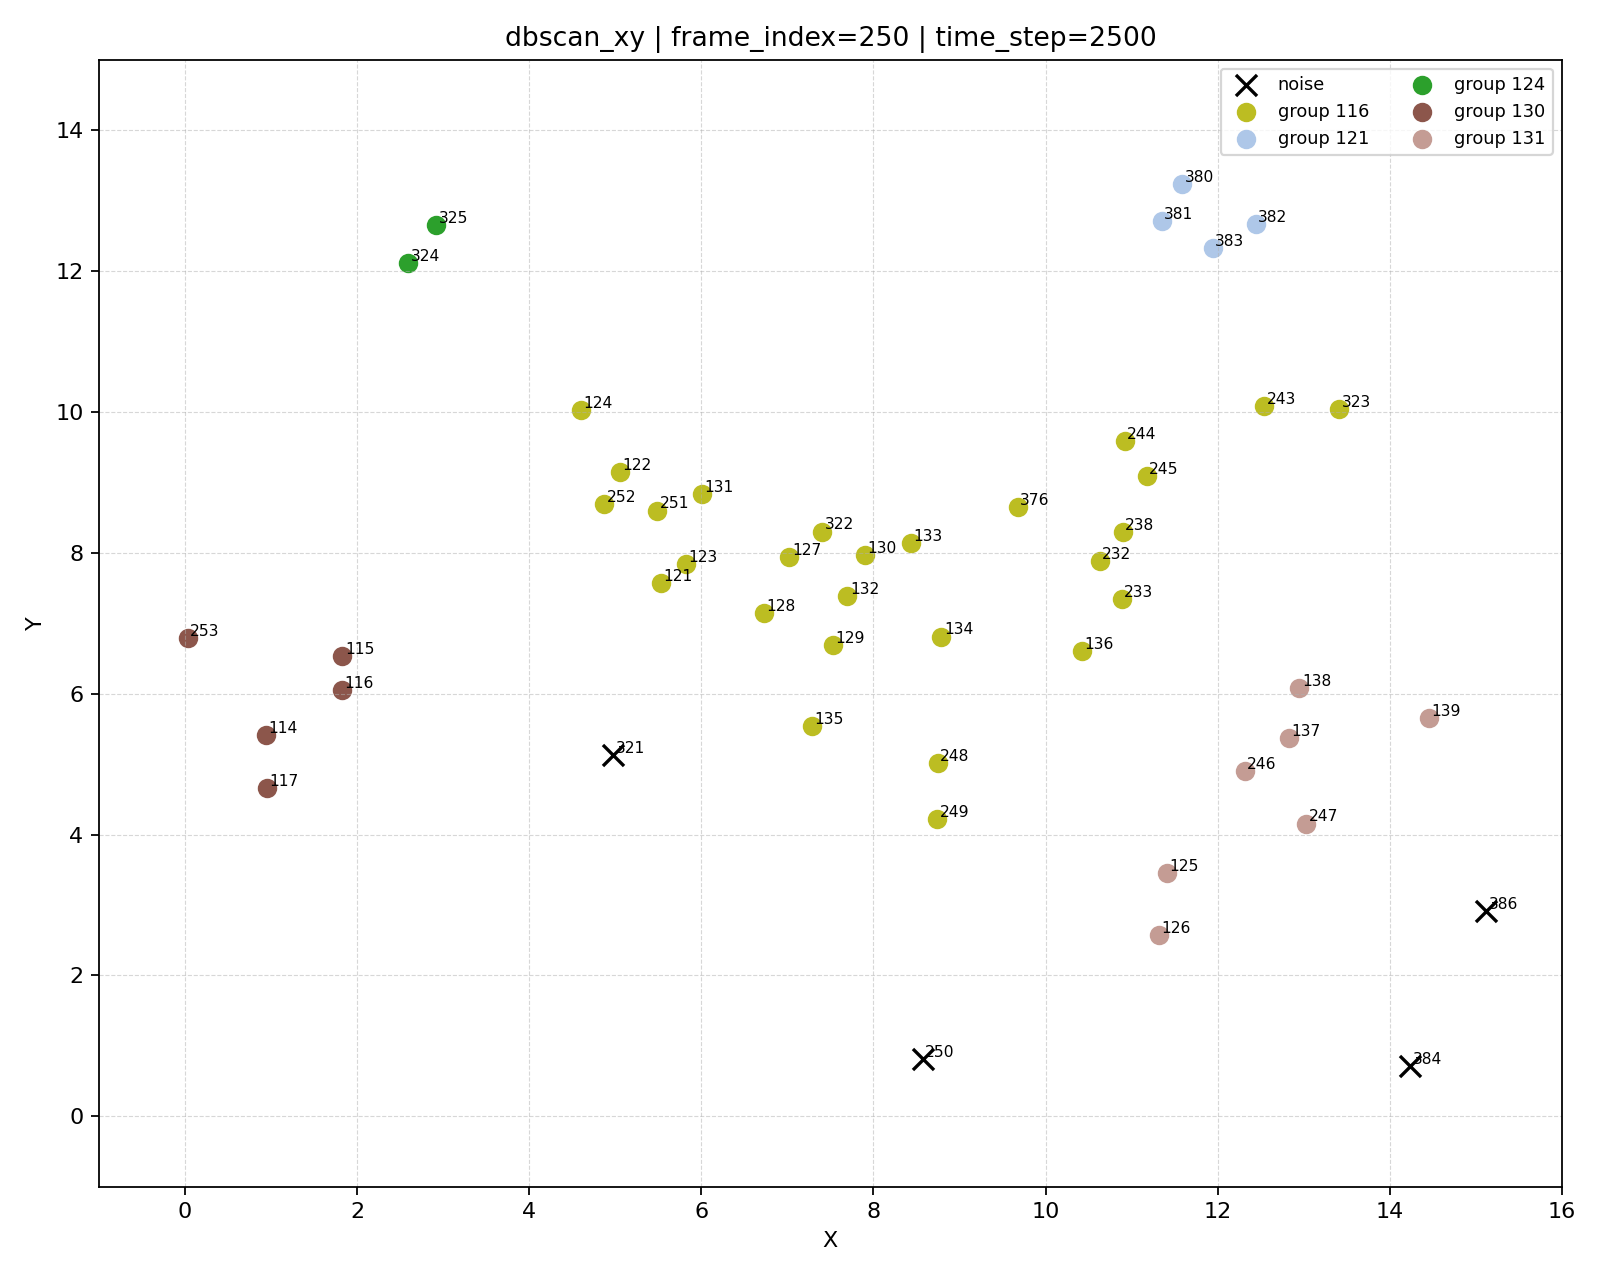
\includegraphics[width=0.78\textwidth]{figures/a_dbscan_frame_0250.png}
\caption{A 类 DBSCAN 在 time\_step=2500 处的聚类结果}
\label{fig:a-dbscan}
\end{figure}

从可视化结果看，A 类 DBSCAN 能够根据空间密度发现若干行人组，但它只利用当前帧空间位置，无法判断行人是否具有持续同行关系。

\subsection{B 类运动特征增强结果}

B 类方法结果表明，运动特征能够增强对不同行人运动差异的区分能力，但运动权重过高时容易导致过度切分。表 \ref{tab:selected-method} 给出了代表方法对比。

\begin{table}[H]
\centering
\caption{代表方法结果对比}
\label{tab:selected-method}
\resizebox{\textwidth}{!}{
\begin{tabular}{llccccc}
\toprule
阶段 & 方法 & 平均簇数 & 最少簇数 & 最多簇数 & 噪声比例 & 至少 2 组比例 \\
\midrule
A & DBSCAN\_spatial & 4.652 & 2 & 8 & 0.077 & 1.000 \\
B & window\_velocity, eps=0.8, mw=1.0 & 7.652 & 2 & 14 & 0.317 & 1.000 \\
B & window\_velocity, eps=1.0, mw=0.5 & 3.954 & 2 & 9 & 0.107 & 1.000 \\
B & momentum, eps=1.0, mw=0.5 & 4.011 & 2 & 9 & 0.103 & 1.000 \\
C & relation\_graph, dt=2.5, vt=0.2 & 4.858 & 2 & 10 & 0.000 & 1.000 \\
C & affinity\_spectral & 3.000 & 3 & 3 & 0.000 & 1.000 \\
\bottomrule
\end{tabular}
}
\end{table}

初始 B 类实验中，\texttt{motion\_weight=1.0} 使运动特征影响较强，导致平均簇数和噪声比例偏高。将 \texttt{eps} 调整为 1.0，并将 \texttt{motion\_weight} 降低为 0.5 后，\texttt{window\_velocity} 方法平均簇数下降至约 3.95，噪声比例下降至约 10.7\%。这说明运动特征应作为空间位置特征的辅助，而不宜完全主导距离度量。

\begin{figure}[H]
\centering

\includegraphics[width=0.78\textwidth]{figures/b_window_velocity_frame_0250.png}
\caption{B 类改进 window\_velocity 方法在 time\_step=2500 处的聚类结果}
\label{fig:b-window}
\end{figure}

\subsection{C 类时序关系建模结果}

C 类方法的核心优势在于显式建模行人之间的持续邻近和运动相似关系。实验中，关系图方法对距离阈值和速度阈值较为敏感。当阈值过严时，图中边较少，容易产生大量小连通分量；适当放宽阈值后，持续同行的人更容易连接成组。

最终，本文选择 \texttt{dist\_threshold=2.5, vel\_threshold=0.20} 作为 C 类关系图代表参数。该方法平均每帧形成约 4.86 个组，但也存在连通分量传递导致过度合并的可能。

\begin{figure}[H]
\centering
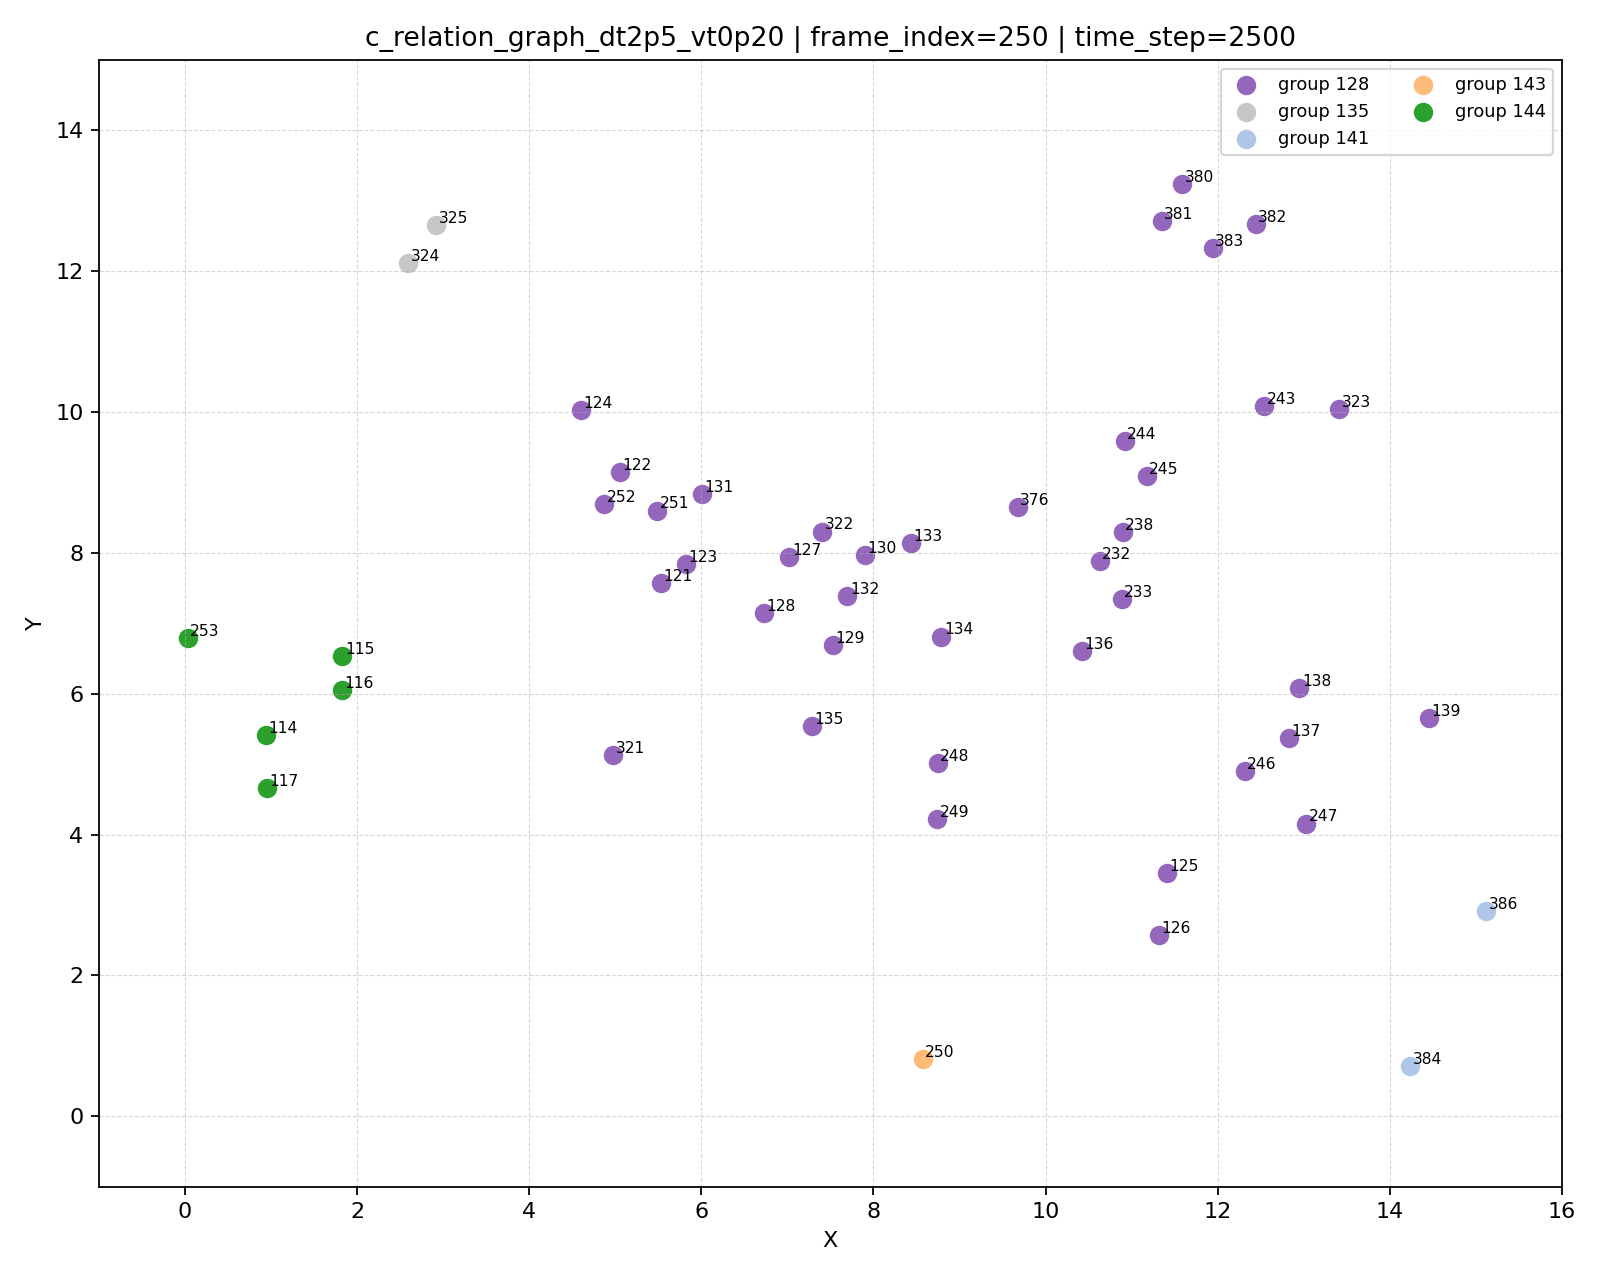
\includegraphics[width=0.78\textwidth]{figures/c_relation_graph_frame_0250.png}
\caption{C 类 relation\_graph 方法在 time\_step=2500 处的聚类结果}
\label{fig:c-graph}
\end{figure}

\subsection{参数与稳定性分析}

图 \ref{fig:avg-clusters} 至图 \ref{fig:stability} 展示了不同方法在平均簇数、噪声比例和连续帧稳定性方面的对比。

\begin{figure}[H]
\centering
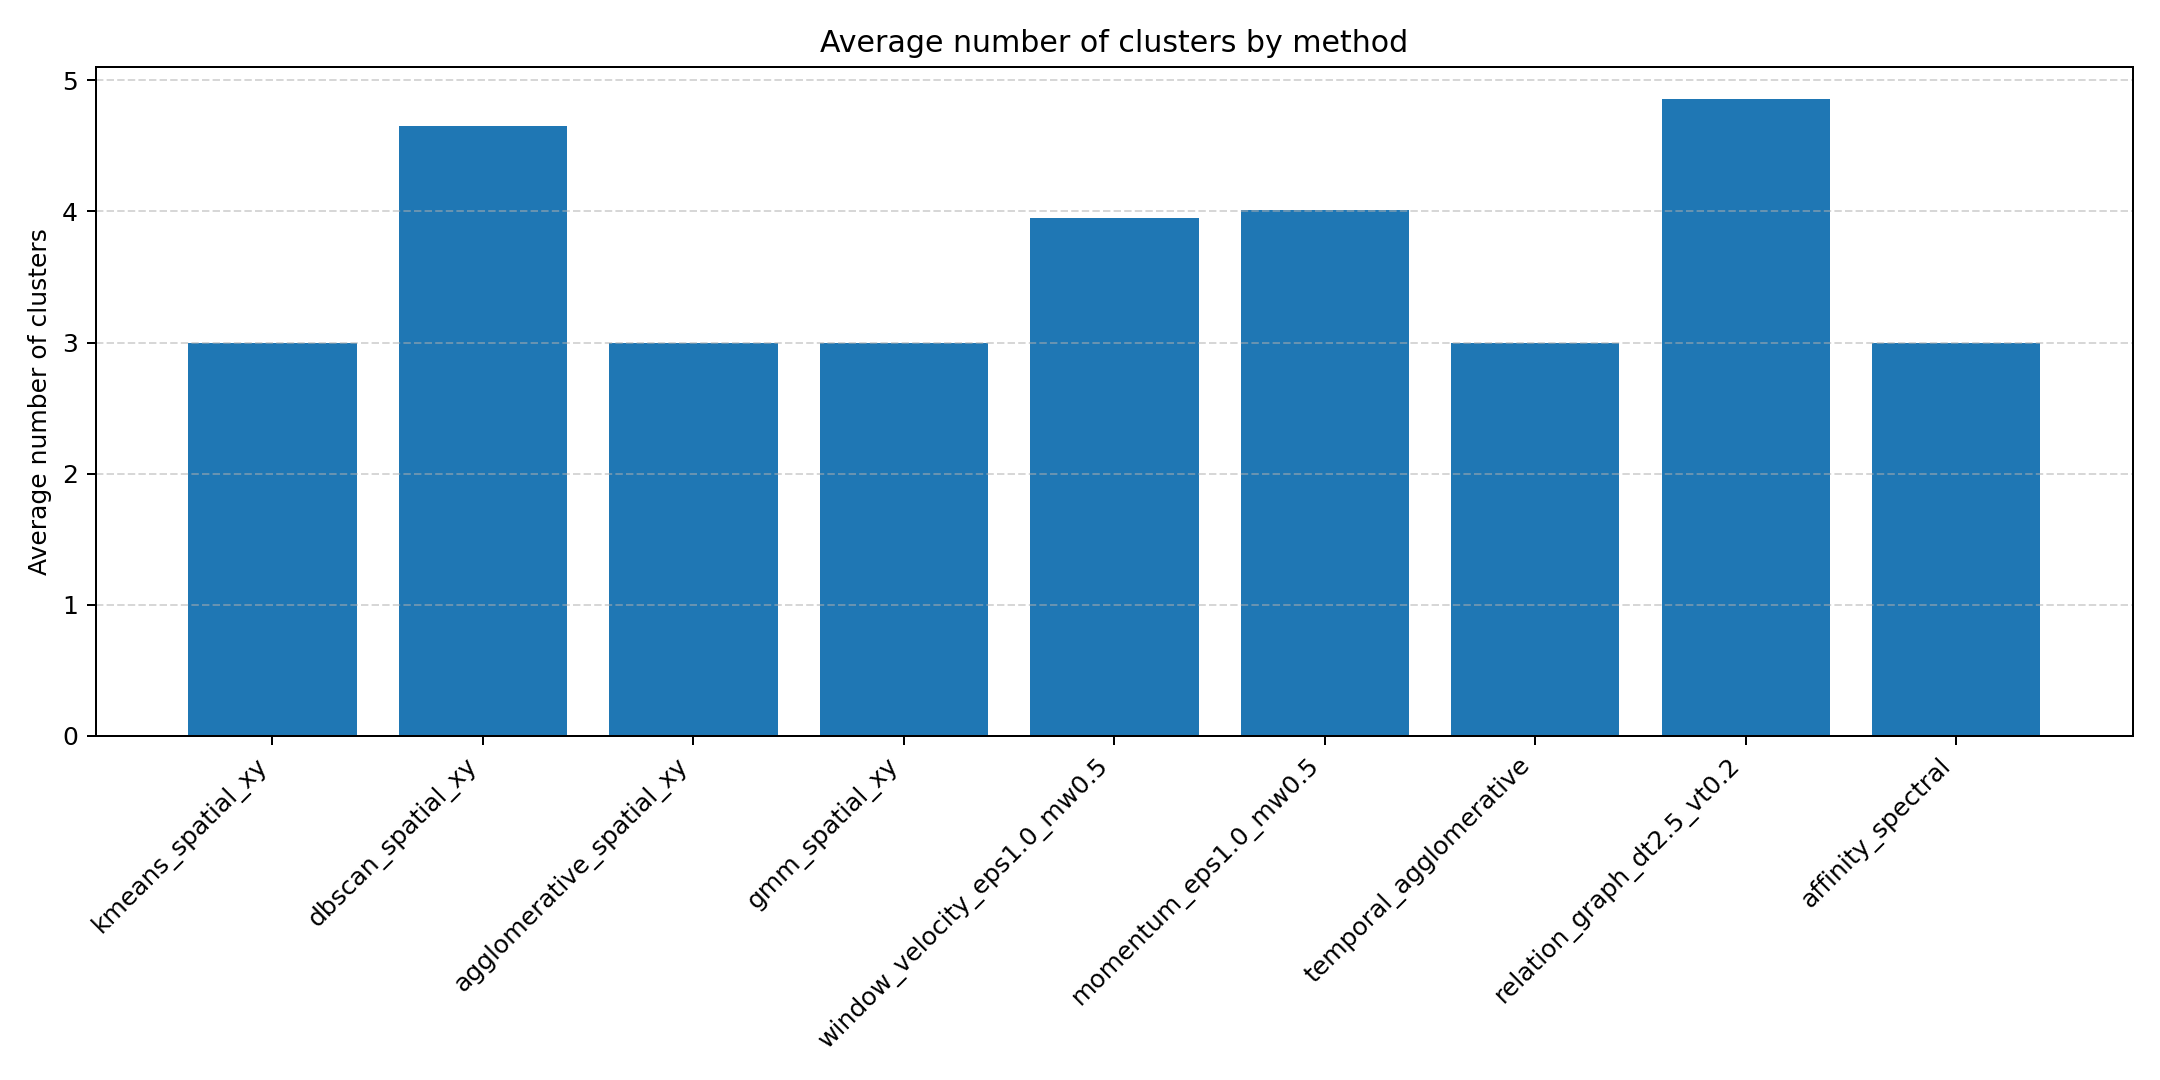
\includegraphics[width=0.9\textwidth]{figures/avg_num_clusters.png}
\caption{不同方法的平均簇数量对比}
\label{fig:avg-clusters}
\end{figure}

\begin{figure}[H]
\centering
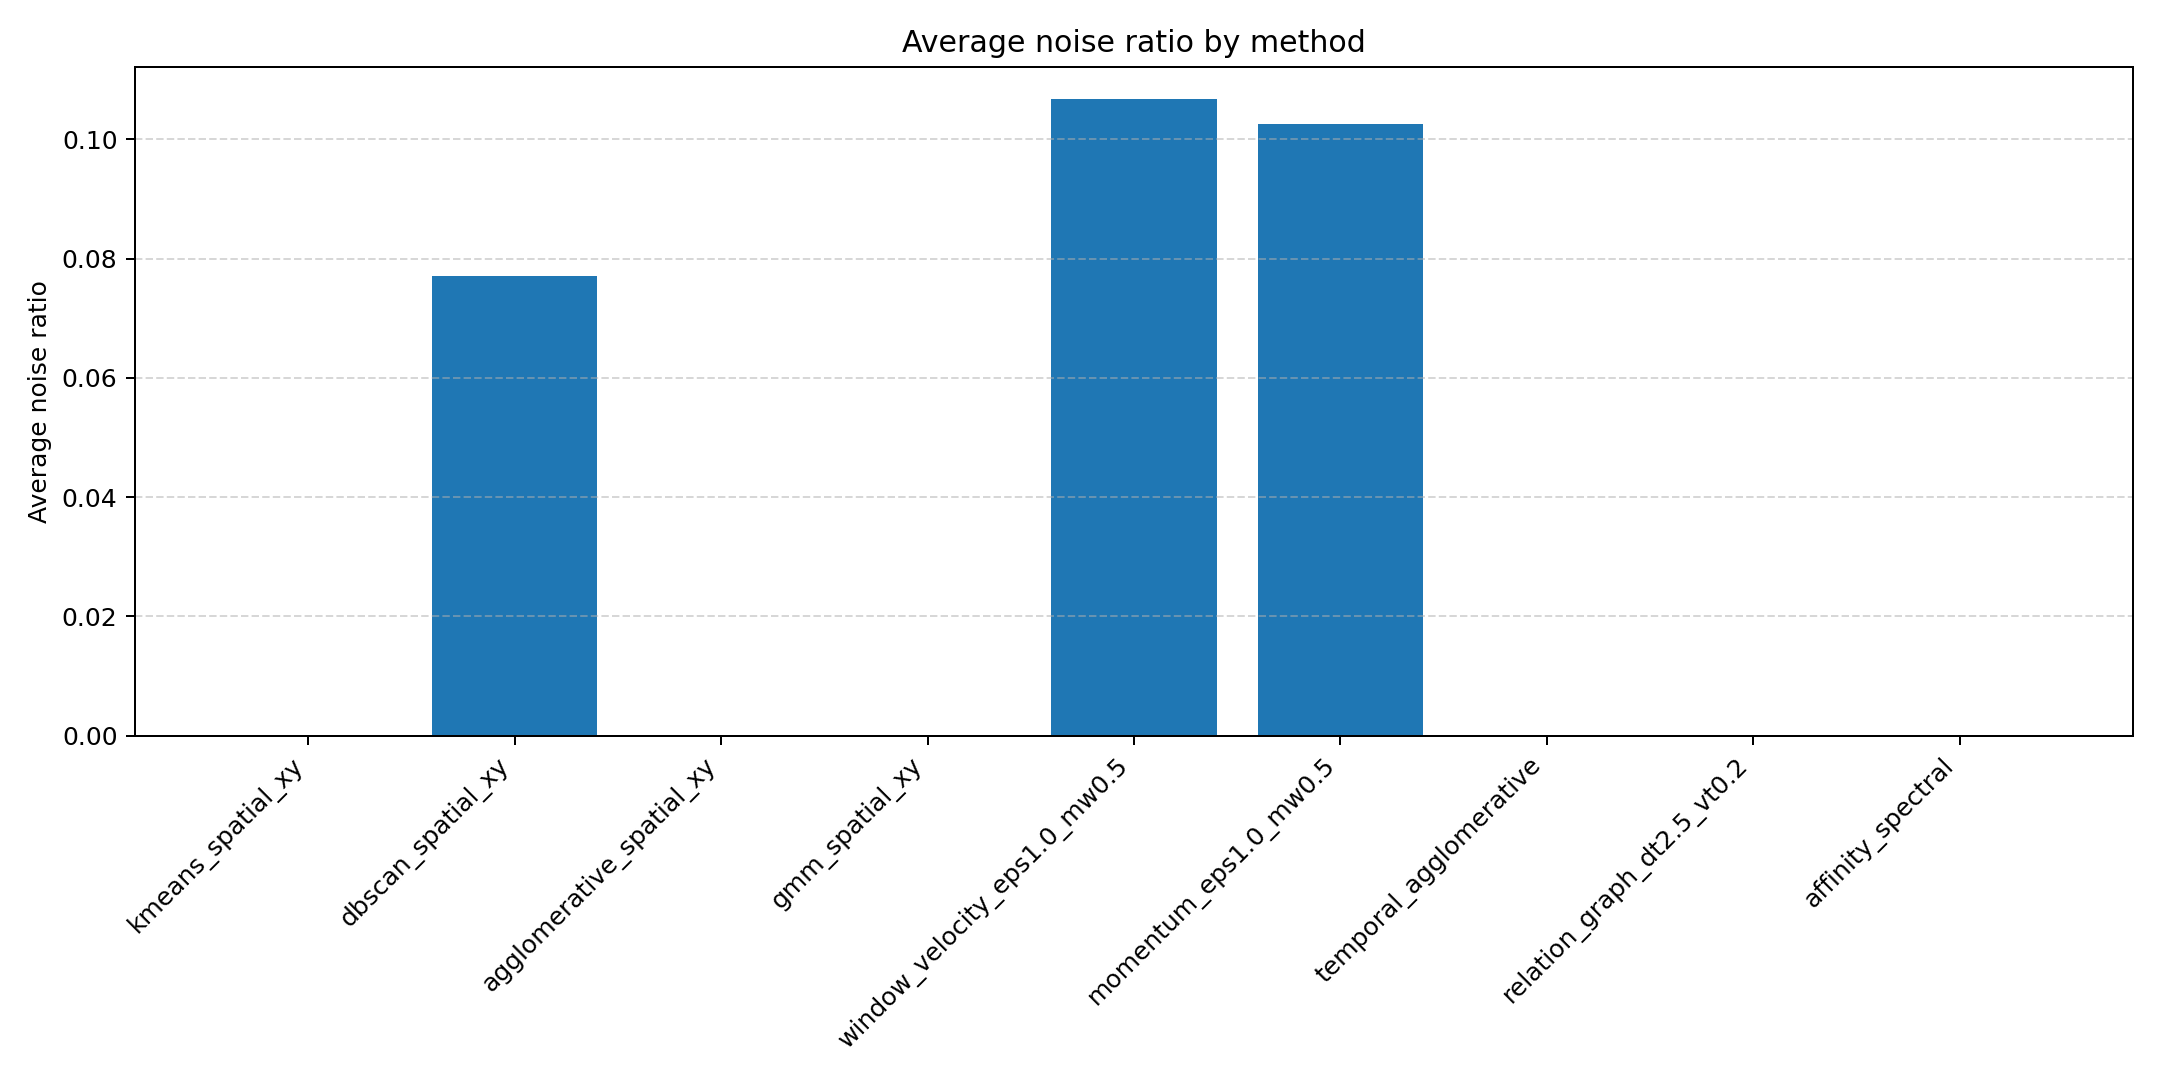
\includegraphics[width=0.9\textwidth]{figures/avg_noise_ratio.png}
\caption{不同方法的平均噪声比例对比}
\label{fig:noise-ratio}
\end{figure}

\begin{figure}[H]
\centering
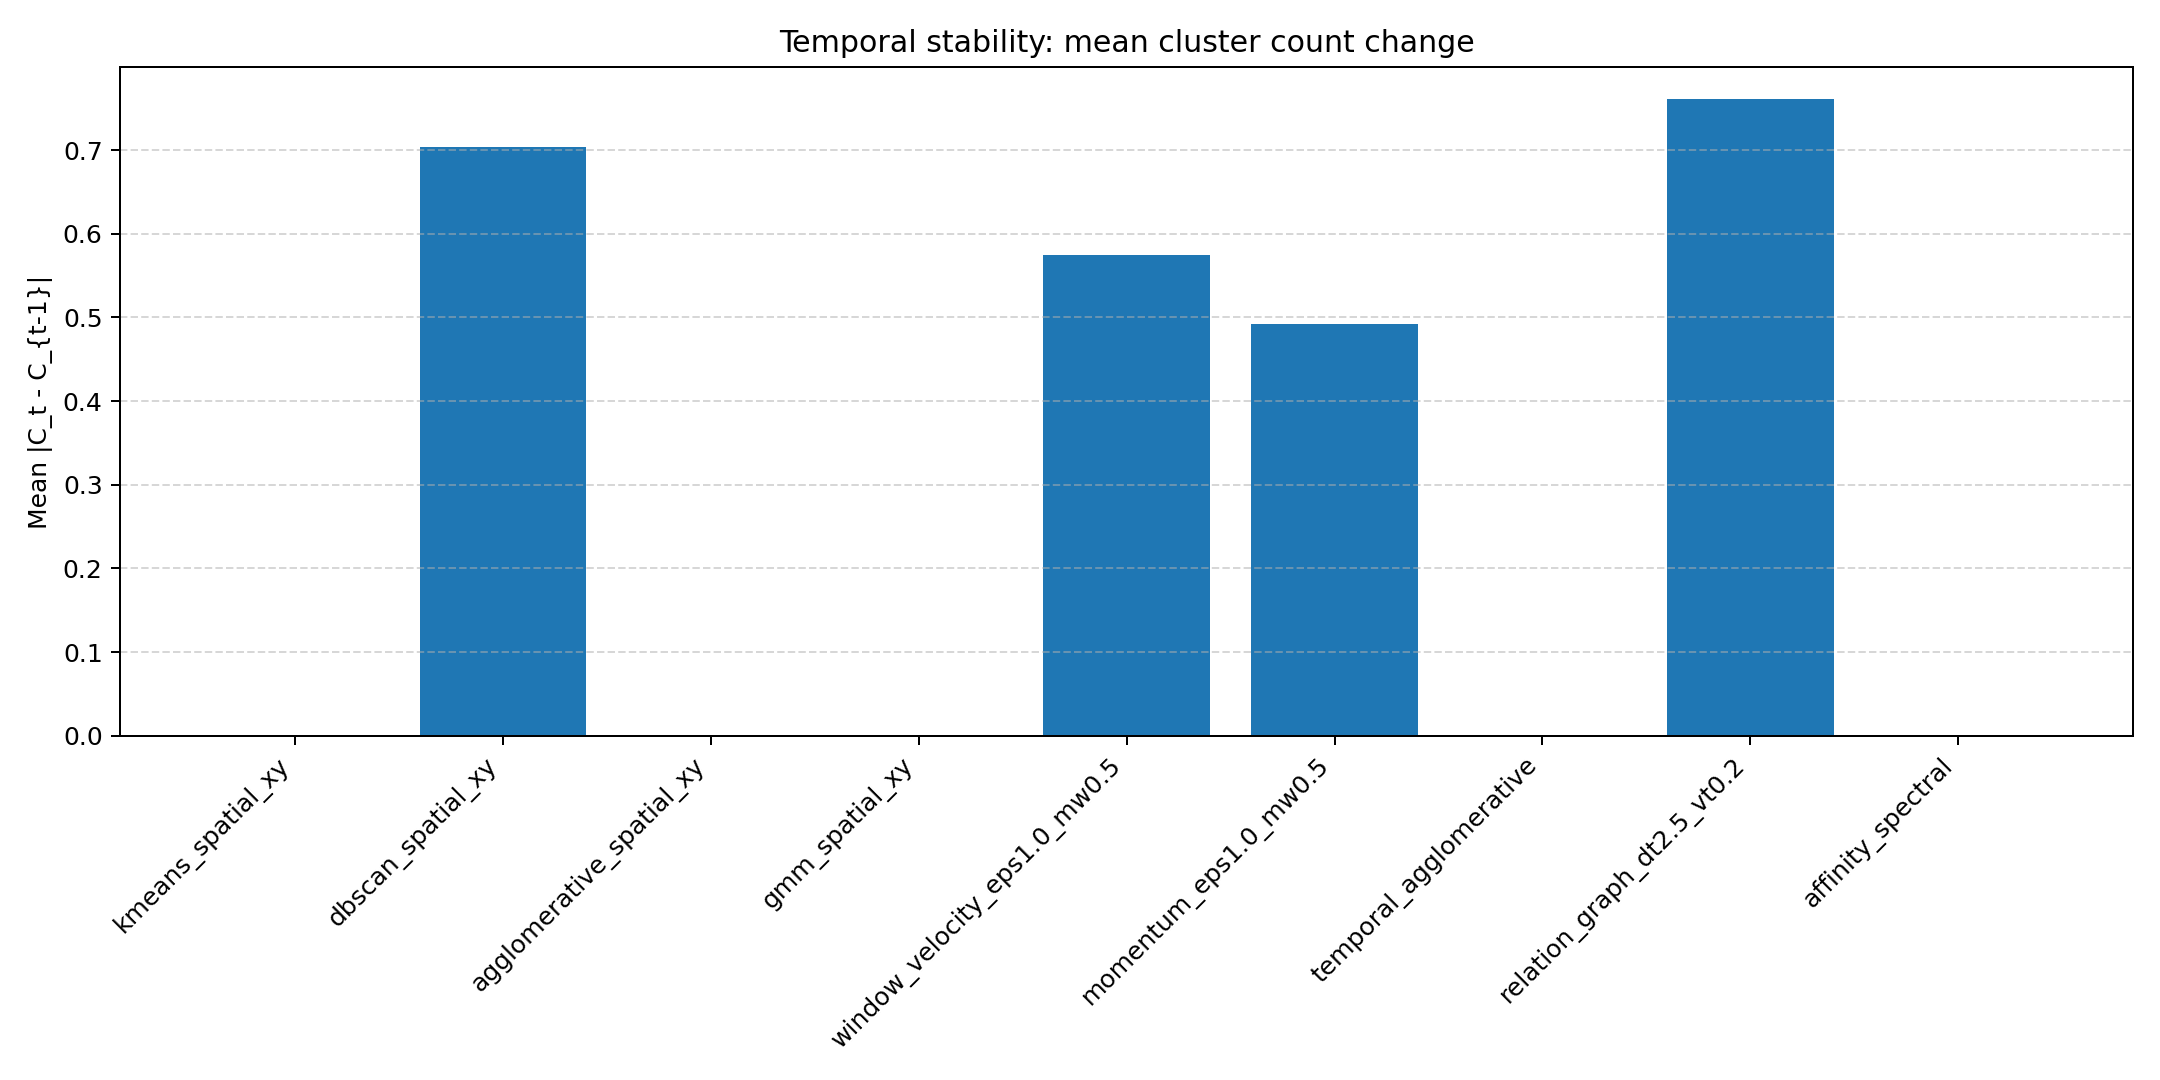
\includegraphics[width=0.9\textwidth]{figures/mean_cluster_count_change.png}
\caption{不同方法的连续帧簇数量变化对比}
\label{fig:stability}
\end{figure}

稳定性统计结果如表 \ref{tab:stability} 所示。

\begin{table}[H]
\centering
\caption{代表方法连续帧稳定性对比}
\label{tab:stability}
\resizebox{\textwidth}{!}{
\begin{tabular}{llccc}
\toprule
阶段 & 方法 & 平均簇数 & 噪声比例 & 平均簇数量变化 \\
\midrule
A & DBSCAN\_spatial & 4.652 & 0.077 & 0.704 \\
B & window\_velocity, eps=0.8, mw=1.0 & 7.652 & 0.317 & 0.791 \\
B & window\_velocity, eps=1.0, mw=0.5 & 3.954 & 0.107 & 0.574 \\
B & momentum, eps=1.0, mw=0.5 & 4.011 & 0.103 & 0.493 \\
C & relation\_graph, dt=2.5, vt=0.2 & 4.858 & 0.000 & 0.761 \\
C & affinity\_spectral & 3.000 & 0.000 & 0.000 \\
\bottomrule
\end{tabular}
}
\end{table}

固定簇数方法在簇数量变化指标上为 0，但这是因为簇数量被人为固定，并不代表其真实分组一定更合理。相较而言，B 类改进方法在保持自动聚类能力的同时，连续帧簇数量变化较低，说明其在稳定性和自适应性之间取得了较好的平衡。

\subsection{Final 最终结果}

在完成 A 类基础空间聚类、B 类运动特征增强、C 类时序关系建模以及参数与稳定性分析后，本文需要从多个候选方案中选择最终视频生成方法。

A 类 DBSCAN 的优点是不需要预先指定簇数，能够根据空间密度自动发现行人组，且噪声比例较低。但是它只使用当前帧 $X,Y$ 坐标，无法利用行人的短时运动趋势，因此容易把空间上接近但运动关系不同的行人合并到同一组。C 类 relation\_graph 方法能够直接建模持续邻近关系，更符合 Group Discovery 的任务直觉，但实验结果表明该方法对距离阈值和速度阈值较为敏感，且连通分量的传递性可能导致局部过度合并。

相比之下，B 类改进后的 window\_velocity 方法在空间位置基础上加入滑动窗口速度，能够利用短时运动趋势；同时通过将 \texttt{motion\_weight} 降低为 0.5，避免了初始运动特征方案中过度切分和噪声比例过高的问题。根据表 \ref{tab:selected-method} 和表 \ref{tab:stability}，该方法平均簇数约为 3.95，平均噪声比例约为 10.7\%，连续帧簇数量变化约为 0.574，在可解释性、稳定性和作业约束之间取得了较好的平衡。虽然改进后的 momentum 方法在连续帧簇数量变化指标上略低，但其指数衰减动量还引入了额外的历史衰减参数，解释和调参成本相对更高；相比之下，滑动窗口速度直接表示最近若干帧的平均运动趋势，更易解释，也更适合作为最终报告中的主方法。因此，本文最终选择 \texttt{window\_velocity + DBSCAN + KMeans fallback} 作为 Final 方法。

最终结果如表 \ref{tab:final-summary} 所示。

\begin{table}[H]
\centering
\caption{Final 方法结果}
\label{tab:final-summary}
\begin{tabular}{lc}
\toprule
指标 & 数值 \\
\midrule
总帧数 & 541 \\
平均簇数 & 3.954 \\
最少簇数 & 2 \\
最多簇数 & 9 \\
簇数标准差 & 1.295 \\
平均噪声比例 & 0.107 \\
fallback 帧数 & 7 \\
fallback 比例 & 0.0129 \\
少于 2 组帧数 & 0 \\
至少 2 组比例 & 1.000 \\
最终视频 & \texttt{final\_group\_discovery.mp4} \\
\bottomrule
\end{tabular}
\end{table}

最终方法覆盖全部 541 帧，且所有帧均至少包含 2 个行人组，满足作业要求。图 \ref{fig:final-frame} 展示了最终方法在关键帧上的可视化结果。

\begin{figure}[H]
\centering
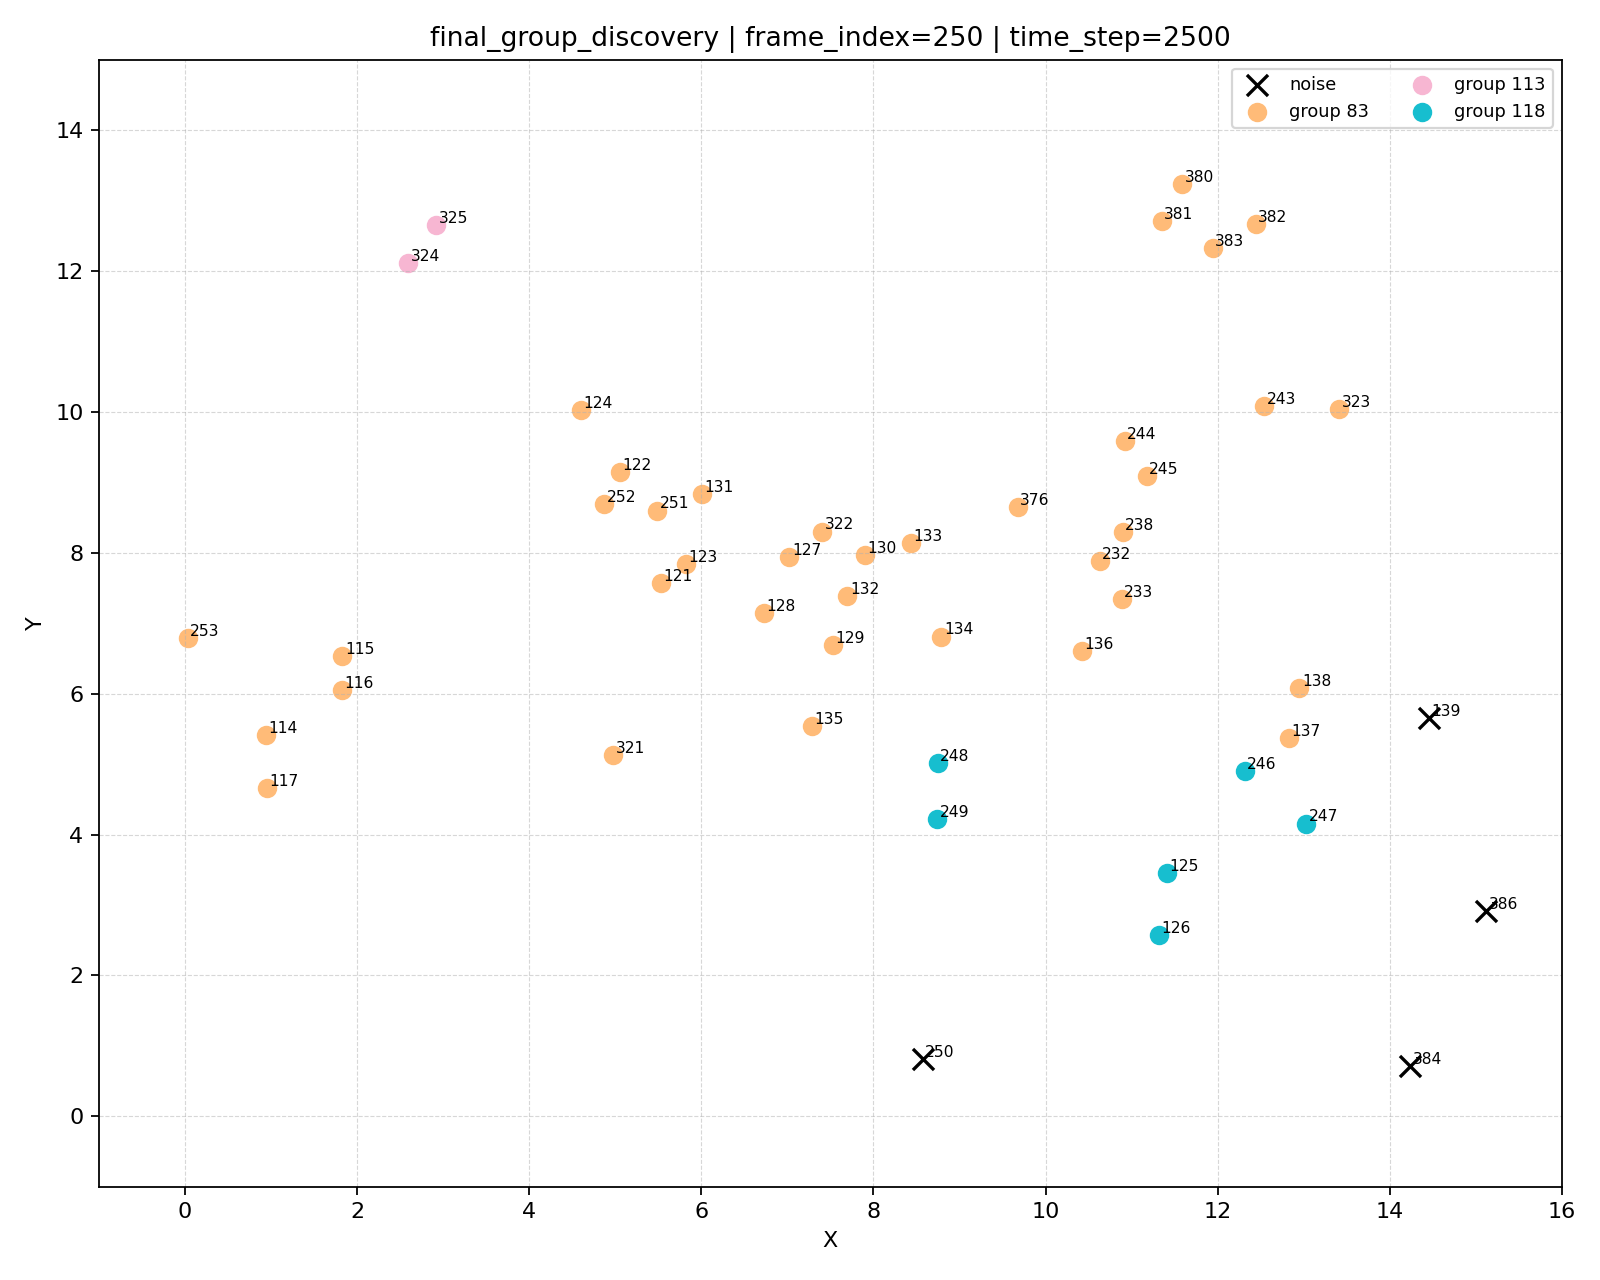
\includegraphics[width=0.78\textwidth]{figures/final_frame_0250.png}
\caption{Final 方法在 time\_step=2500 处的行人组发现结果}
\label{fig:final-frame}
\end{figure}

从图中可以看到，Final 方法能够用不同颜色表示不同组，并用黑色叉号表示 DBSCAN 判定的噪声点。该帧中部区域存在较大的行人组，说明 DBSCAN 在局部密度连续时可能将多个相邻小组合并为较大组。这体现了最终方法在稳定性、噪声控制和细粒度分组之间的折中。

最终视频文件为 \texttt{outputs/final/video/final\_group\_discovery.mp4}，视频由 541 张逐帧可视化图片按 10 fps 合成，能够连续展示 students003 数据从 \texttt{time\_step=0} 到 \texttt{time\_step=5400} 的行人组发现结果。

\section{关键代码说明}

本节仅展示实验中的核心代码片段，完整工程代码保存在实验目录中。

\subsection{数据读取与逐帧组织}

\lstinputlisting[caption={数据读取与逐帧组织代码},label={code:data-loading}]{code/data_loading.py}

该代码负责读取 students003 数据，并按照 \texttt{time\_step} 逐帧组织行人点，为后续逐帧聚类提供基础。

\subsection{运动特征构造}

\lstinputlisting[caption={运动特征构造代码},label={code:motion-features}]{code/motion_features.py}

该代码计算瞬时速度、滑动窗口速度、指数动量和运动方向特征，是 B 类运动特征增强方法的核心。

\subsection{DBSCAN + KMeans 兜底策略}

\lstinputlisting[caption={DBSCAN + KMeans 兜底代码},label={code:dbscan-fallback}]{code/dbscan_fallback.py}

该代码首先使用 DBSCAN 自动发现组数；若某帧有效组数少于 2，则使用 KMeans 兜底，从而满足作业中每帧至少 2 组的要求。

\subsection{关系图方法}

\lstinputlisting[caption={基于关系图的时序关系建模代码},label={code:temporal-relation}]{code/temporal_relation.py}

该代码根据两名行人的平均空间距离和平均速度差建立关系图，并将连通分量作为行人组。

\subsection{可视化与视频生成}

\lstinputlisting[caption={逐帧可视化与视频生成代码},label={code:visualization}]{code/visualization.py}

该代码负责将每一帧的聚类结果绘制为 PNG 图片，并使用 ffmpeg 合成 MP4 视频。

\section{总结与不足}

本文围绕 students003 行人轨迹数据完成了 Group Discovery 实验。实验从基础空间聚类出发，逐步加入运动特征和时序关系建模，并通过参数分析和连续帧稳定性评价选择最终方法。最终采用基于滑动窗口速度特征的 DBSCAN + KMeans 兜底策略，成功生成完整视频，并保证全部 541 帧均至少包含 2 个行人组。

本文的主要工作包括：

\begin{enumerate}
    \item 完成 students003 数据格式检查，确认数据适合逐帧聚类；
    \item 实现 KMeans、DBSCAN、Agglomerative Clustering 和 GMM 四种 A 类 baseline；
    \item 实现瞬时速度、滑动窗口速度、指数动量和方向特征四类 B 类方法；
    \item 实现持续邻近关系、关系图和 pairwise affinity 谱聚类三类 C 类方法；
    \item 进行参数分析、稳定性评价和可视化对比；
    \item 生成最终逐帧可视化图片和 MP4 视频。
\end{enumerate}

实验也存在不足。首先，数据没有真实行人组标签，因此评价主要依赖无监督指标和可视化分析，无法计算严格的监督准确率。其次，DBSCAN 和关系图方法对参数较敏感，不同参数会影响过度切分或过度合并。再次，滑动窗口速度只能近似表达短时运动趋势，不能完全判断真实社交关系。未来可以进一步引入轨迹级聚类、图社区发现、跨帧组身份跟踪以及人工标注评价，从而提高 Group Discovery 的可靠性和可解释性。

\appendix

\section{主要输出文件}

本实验主要输出文件如下：

\begin{itemize}
    \item \texttt{outputs/final/clusters\_final.csv}：最终逐帧聚类结果；
    \item \texttt{outputs/final/stats\_final.csv}：最终逐帧统计结果；
    \item \texttt{outputs/final/final\_summary.csv}：最终方法总体指标；
    \item \texttt{outputs/final/frames/}：最终逐帧可视化图片；
    \item \texttt{outputs/final/video/final\_group\_discovery.mp4}：最终视频；
    \item \texttt{outputs/final/report\_figures/}：最终报告关键帧。
\end{itemize}

\end{document}
